\documentclass[11pt,a4paper]{article}

\usepackage[utf8]{inputenc}
\usepackage[T1]{fontenc}
\usepackage[spanish,es-noquoting]{babel}
\usepackage[margin=2.4cm]{geometry}
\usepackage{booktabs}
\usepackage{graphicx}
\usepackage{xcolor}
\usepackage{pgfplots}
\pgfplotsset{compat=1.17}
\usepackage[hidelinks]{hyperref}

\graphicspath{{screenshots/}}
\setlength{\parskip}{0.5em}
\setlength{\parindent}{0pt}

\title{\vspace{-1.5cm}\textbf{Búsqueda de Ruta Mínima en Grafos con OpenMP}\\[0.3em]
\large Examen Parcial 1 --- Computación Paralela}

\author{\textbf{Consultora HPC: Tres Punto Uno Cuatro}\\[0.6em]
Anthony Lou Schwank \quad\textbullet\quad Christa Isabella Obando}

\date{11 de septiembre de 2026\\[0.4em]
\small\url{https://github.com/anthonylouschwank/Parcial1-Paralela}}

\begin{document}
\maketitle

%=============================================================================
\section{Contexto y datos}

\subsection*{El problema}

Dada una red social de millones de usuarios (nodos) y sus amistades (aristas),
hay que encontrar el camino más corto de conexiones entre un Usuario X y un
Usuario Y, explorando vecinos paso a paso mediante una cola de tareas
pendientes.

La dificultad no es el algoritmo, que es un BFS de libro. Es el
\textbf{desbalance de carga}: en una red social los grados siguen una ley de
potencias. Casi todos los usuarios tienen un puñado de amigos, pero unos pocos
\emph{hubs} tienen decenas de miles. Repartir la exploración ingenuamente deja
a un hilo terminando en microsegundos mientras otro procesa solo las 10\,000
amistades de un influencer.

\subsection*{Propuesta secuencial}

Implementamos dos variantes en \texttt{/secuencial}:

\begin{enumerate}
\item \textbf{BFS de cola} (\texttt{bfs\_cola}): el algoritmo de libro con
      \texttt{std::queue}. Es la ``cola de tareas pendientes'' literal del
      enunciado y sirve como referencia de correctitud.
\item \textbf{BFS por frontera} (\texttt{bfs\_frontera}): la misma exploración,
      pero la cola se reorganiza en \emph{frontera actual} y \emph{frontera
      siguiente}. Dentro de un nivel los usuarios son independientes entre sí,
      y ahí está el paralelismo.
\end{enumerate}

La segunda es la \emph{baseline} contra la que medimos el speedup, porque es el
mismo algoritmo que corre la versión paralela. Comparar contra otra cosa
inflaría el resultado artificialmente.

\subsection*{Justificación de los datos de prueba}

\textbf{Origen.} Generamos la red con el modelo de conexión preferente de
Barabási--Albert: cada usuario nuevo elige amigos con probabilidad proporcional
a los que ya tienen. Preferimos esto a descargar un dataset real por dos
razones prácticas: la semilla fija (314) garantiza que todas las máquinas midan
sobre la red \emph{idéntica}, y podemos escalar el tamaño a voluntad. El
generador vive en \texttt{/comun}, compartido por ambas implementaciones, para
que no haya forma de que midan sobre grafos distintos.

\textbf{Tamaño.} 2\,000\,000 de usuarios y 15\,999\,964 amistades. El CSR ocupa
137.3~MB.

\textbf{¿Reproduce el fenómeno?} Sí, y está medido, no supuesto:

\begin{center}
\begin{tabular}{lrrrrr}
\toprule
& Mínimo & Mediana & Promedio & p99 & \textbf{Máximo} \\
\midrule
Amistades por usuario & 8 & 11 & 16.0 & 84 & \textbf{6\,414} \\
\bottomrule
\end{tabular}
\end{center}

El 1\% de usuarios más conectados concentra el 10.5\% de las amistades, y la
razón máximo/mediana es de \textbf{583$\times$}. Ese es exactamente el
desbalance que hay que vencer. Con 5\,000\,000 de usuarios el hub máximo llega
a \textbf{10\,249} amigos, el número literal del enunciado.

\textbf{Estructura en memoria.} Grafo no dirigido en formato \textbf{CSR}
(\emph{Compressed Sparse Row}): un arreglo \texttt{offsets} de tamaño $n+1$ y
uno \texttt{ady} de tamaño $2m$ con toda la adyacencia contigua. Frente a un
\texttt{vector<vector<int>>}, CSR evita dos millones de asignaciones dispersas
en el heap y un fallo de caché por cada salto de nodo. Además es de solo
lectura durante el BFS, así que todos los hilos la comparten sin ninguna
sincronización.

%=============================================================================
\section{Estrategia de paralelización}

\subsection*{Directivas utilizadas}

\textbf{\texttt{\#pragma omp parallel}, una sola vez para todo el BFS.}
Nuestra primera versión abría y cerraba una región paralela \emph{por nivel}.
Los niveles 0--2 mueven apenas unos miles de aristas, pero costaban 20~ms con 8
hilos contra 0.45~ms con 1: puro costo de arrancar y dormir el equipo de hilos.
Ahora el equipo se crea una vez y los niveles se separan con barreras, que son
órdenes de magnitud más baratas.

\textbf{\texttt{\#pragma omp for schedule(runtime)}} sobre la frontera. Cada
iteración expande un usuario, y su costo es proporcional a su número de amigos,
que varía en tres órdenes de magnitud. Usamos \texttt{runtime} y no una
política fija para que las tres alternativas recorran exactamente el mismo
código máquina: así la comparación entre ellas mide la política y no
diferencias de compilación.

\textbf{\texttt{\#pragma omp single} y \texttt{\#pragma omp barrier}} para
cerrar cada nivel: calcular desplazamientos, intercambiar fronteras y decidir
si continuar.

\subsection*{Cómo evitamos las condiciones de carrera}

Dos hilos pueden descubrir al mismo usuario $w$ en el mismo instante. Si ambos
leen \texttt{visitado[w] == 0} y ambos lo encolan, $w$ entra duplicado en la
frontera y \texttt{padre[w]} queda indefinido.

La solución es un \textbf{compare-and-swap atómico} sobre
\texttt{visitado[w]}. Exactamente un hilo logra la transición $0 \to 1$; ese es
el único que escribe \texttt{padre[w]} y encola. Es indivisible: no hay ventana
entre ``leo que está libre'' y ``lo marco como mío''. Lo precede una lectura
relajada como filtro barato, porque la enorme mayoría de vecinos ya fueron
visitados y no vale la pena pagar el CAS.

Un segundo punto de contención es la construcción de la frontera siguiente. Si
todos los hilos hicieran \texttt{push\_back} sobre un vector compartido --- o
peor, dentro de un \texttt{critical} --- se serializarían millones de
inserciones por nivel. En vez de eso \textbf{cada hilo acumula en su propio
buffer local}, sin sincronización alguna, y al cerrar el nivel se calculan los
desplazamientos y cada hilo copia su bloque en paralelo a un rango disjunto.

\textbf{Verificación.} El programa comprueba en cada corrida que el camino
hallado sea real (cada salto debe ser una amistad existente) y que las
invariantes --- usuarios visitados y amistades recorridas --- no varíen entre
repeticiones. Si hubiera una carrera sin resolver, variarían. En las 52
corridas de las dos máquinas no varió ninguna.

Sí cambia el \emph{camino} entre corridas, y es correcto: gana el hilo que
consiga el CAS, y es él quien queda como padre. La \emph{longitud} nunca
cambia.

\subsection*{Cómo atacamos el desbalance de carga}

Probamos las tres políticas de OpenMP con cuatro tamaños de bloque, en las dos
máquinas, con 8 hilos:

\begin{center}
\begin{tabular}{llrr}
\toprule
\textbf{Scheduling} & \textbf{Chunk} & \textbf{i5-1035G1 (ms)} & \textbf{i7-11370H (ms)} \\
\midrule
static  & default & 140.44 & 136.06 \\
static  & 16      & 141.02 & 121.31 \\
static  & 64      & 150.87 & 130.05 \\
static  & 256     & 162.74 & 180.34 \\
dynamic & default & 152.76 & 140.17 \\
\textbf{dynamic} & \textbf{16} & \textbf{130.18} & \textbf{109.64} \\
dynamic & 64      & 139.03 & 112.04 \\
dynamic & 256     & 172.32 & 112.41 \\
guided  & default & 143.61 & 119.12 \\
guided  & 16      & 143.53 & 124.33 \\
guided  & 64      & 148.30 & 117.52 \\
guided  & 256     & 144.76 & 128.78 \\
\bottomrule
\end{tabular}
\end{center}

\textbf{\texttt{dynamic} con chunk 16 gana en las dos máquinas de forma
independiente}, por 7.9\% sobre el mejor \texttt{static} en la i5 y 10.6\% en
la i7. Un resultado replicado en hardware distinto es mucho más sólido que uno
medido una sola vez. El chunk pequeño importa: con 256 el reparto se vuelve
grueso y \texttt{dynamic} pierde contra \texttt{static}.

\textbf{Un matiz honesto.} La ganancia es real pero modesta, y conviene decir
por qué. En los niveles dominantes la frontera tiene más de un millón de
usuarios; repartida entre 8 hilos, la varianza de los grados se promedia sola.
El desbalance muerde en los niveles intermedios: en el nivel 3 medimos
1.45$\times$ de desbalance incluso con \texttt{dynamic}, y hasta 2.06$\times$
en el nivel 2 con \texttt{static}.

Además, nuestra métrica de desbalance (aristas del hilo más cargado sobre el
promedio) \emph{engaña} con \texttt{dynamic}: llega a marcar 1.38$\times$
contra 1.09$\times$ de \texttt{static} y aun así \texttt{dynamic} gana de punta
a punta. La razón es que \texttt{dynamic} no iguala aristas asignadas, iguala
\textbf{tiempo}: un hilo que corre más lento toma menos bloques, que es
exactamente lo que debe pasar.

%=============================================================================
\section{Resultados y métricas}

\subsection*{Metodología}

Ambos binarios se compilan con banderas idénticas (\texttt{-O3 -std=c++17});
la única diferencia es \texttt{-fopenmp}. Se reporta la \textbf{mediana} de 7
repeticiones, no el promedio, porque en una laptop cualquier tarea del sistema
operativo produce valores atípicos.

Entre configuraciones hay una \textbf{pausa de 30 segundos}. Medirlo nos costó
una tarde: sin la pausa, la misma configuración daba 132~ms en frío y 316~ms
tras diez minutos de carga sostenida. Sin enfriar, la curva de escalabilidad
mide la disipación térmica del equipo, no el algoritmo.

Cada corrida deja su salida completa en
\texttt{docs/resultados/<máquina>/salidas/}, y los tiempos crudos en
\texttt{mediciones.csv} (196 filas por máquina).

\subsection*{Escenario principal: recorrido completo de la red}

Las dos versiones recorren exactamente las mismas 31\,999\,928 amistades y
visitan los 2\,000\,000 de usuarios, así que la comparación es limpia.

\vspace{0.5em}
\begin{minipage}[t]{0.48\textwidth}
\textbf{Christa Isabella Obando Guzman --- Intel i5-1035G1}\\
{\footnotesize 4 núcleos físicos / 8 hilos lógicos, 15~W. Baseline secuencial:
\textbf{342.54~ms}.}
\begin{center}\footnotesize
\begin{tabular}{rrrr}
\toprule
Hilos & Mediana & Speedup & Efic. \\
\midrule
1 & 400.91 & 0.85$\times$ & 85\% \\
2 & 224.33 & 1.53$\times$ & 76\% \\
3 & 184.66 & 1.85$\times$ & 62\% \\
4 & 158.79 & 2.16$\times$ & 54\% \\
6 & \textbf{137.04} & \textbf{2.50$\times$} & 42\% \\
8 & 144.89 & 2.36$\times$ & 30\% \\
\bottomrule
\end{tabular}
\end{center}
\end{minipage}
\hfill
\begin{minipage}[t]{0.48\textwidth}
\textbf{Anthony Lou Schwank --- Intel i7-11370H}\\
{\footnotesize 4 núcleos físicos / 8 hilos lógicos, 35~W. Baseline secuencial:
\textbf{369.19~ms}.}
\begin{center}\footnotesize
\begin{tabular}{rrrr}
\toprule
Hilos & Mediana & Speedup & Efic. \\
\midrule
1 & 449.46 & 0.82$\times$ & 82\% \\
2 & 240.40 & 1.54$\times$ & 77\% \\
3 & 185.71 & 1.99$\times$ & 66\% \\
4 & 156.34 & 2.36$\times$ & 59\% \\
6 & 122.22 & 3.02$\times$ & 50\% \\
8 & \textbf{114.86} & \textbf{3.21$\times$} & 40\% \\
\bottomrule
\end{tabular}
\end{center}
\end{minipage}

\begin{center}
\begin{tikzpicture}
\begin{axis}[
    width=12cm, height=7cm,
    xlabel={Hilos}, ylabel={Speedup vs.\ secuencial},
    xtick={1,2,3,4,6,8}, ymin=0, xmin=0.6, xmax=8.4,
    grid=major, grid style={gray!25},
    legend pos=north west, legend cell align=left,
    tick label style={font=\small}, label style={font=\small},
    legend style={font=\small}
]
\addplot[dashed, gray, thick, domain=1:8, samples=2] {x};
\addlegendentry{Ideal (lineal)}
\addplot[color=blue!70!black, mark=*, thick]
    coordinates {(1,0.85)(2,1.53)(3,1.85)(4,2.16)(6,2.50)(8,2.36)};
\addlegendentry{i5-1035G1}
\addplot[color=red!70!black, mark=square*, thick]
    coordinates {(1,0.82)(2,1.54)(3,1.99)(4,2.36)(6,3.02)(8,3.21)};
\addlegendentry{i7-11370H}
\end{axis}
\end{tikzpicture}
\end{center}

\subsection*{Lectura de los resultados}

\textbf{Con 1 hilo el speedup es menor a 1} (0.85$\times$ y 0.82$\times$). Es
el costo de arrastrar el runtime de OpenMP sin ningún beneficio, y explica de
dónde parte la curva.

\textbf{La eficiencia cae porque se acaban los núcleos, no porque falle el
reparto.} Ambas máquinas tienen 4 núcleos físicos; más allá de ese número los
hilos comparten unidades de ejecución (SMT) y no hay más núcleos entre los que
repartir. A 4 hilos la eficiencia es 54\% y 59\%.

\textbf{Mismo paralelismo, techo distinto.} Las dos máquinas tienen idéntico
número de núcleos, pero la i5 hace pico en 6 hilos y \emph{empeora} con 8,
mientras la i7 sigue mejorando. Como el grado de paralelismo es el mismo, la
diferencia no puede ser del algoritmo: es ancho de banda de memoria y
frecuencia sostenida. Esto confirma que el BFS aquí está limitado por memoria y
no por cómputo, algo que detectamos en la versión inicial al medir nivel por
nivel: el nivel dominado por escrituras escalaba 1.19$\times$ mientras el
dominado por lecturas escalaba 1.87$\times$.

\subsection*{Limitación medida: la consulta X $\to$ Y}

En la consulta puntual del enunciado nuestra versión paralela \textbf{pierde}
contra el BFS de cola secuencial:

\begin{center}
\begin{tabular}{lrrr}
\toprule
& \textbf{BFS de cola} & \textbf{Paralelo} & \textbf{Speedup} \\
& \textbf{(1 hilo)} & \textbf{(8 hilos)} & \textbf{real} \\
\midrule
i5-1035G1 & 49.66~ms & 59.97~ms & 0.83$\times$ \\
i7-11370H & 37.73~ms & 52.91~ms & 0.71$\times$ \\
\bottomrule
\end{tabular}
\end{center}

La causa está medida. El BFS de cola abandona \emph{en el instante} en que
descubre el destino, a media capa, y recorre 1\,599\,662 aristas. Nuestra
versión por frontera debe cerrar el nivel completo antes de poder revisar, y
ese nivel es justo donde la frontera explota: recorre 12\,450\,125 aristas,
\textbf{7.8$\times$ más trabajo}. Paralelizar 3$\times$ no alcanza para
recuperar 7.8$\times$.

Contra su propia baseline por frontera el paralelismo sí funciona
(3.03$\times$ en la i5, 2.58$\times$ en la i7), pero preferimos reportar la
comparación desfavorable: el speedup honesto se mide contra el mejor secuencial
disponible, no contra el más conveniente.

\textbf{Cómo se arreglaría.} Añadir corte anticipado a media capa también en la
versión paralela, con una bandera atómica que los hilos consulten para
abandonar el resto de su bloque. El costo es que el trabajo deja de ser
determinista --- cada corrida recorrería un número distinto de aristas según
qué hilo encuentre primero el destino --- y habría que relajar la verificación
de invariantes para ese modo. No lo implementamos por tiempo; queda
documentado y medido.

\subsection*{Evidencia de ejecución}

\begin{figure}[h]
\centering
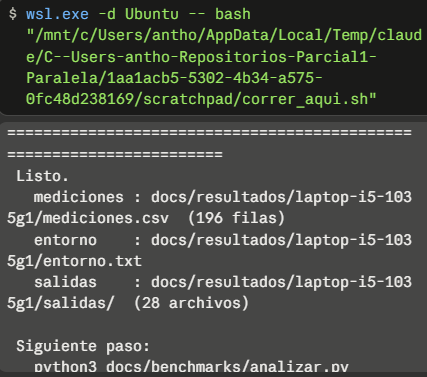
\includegraphics[width=0.60\textwidth]{i5.png}\\[1em]
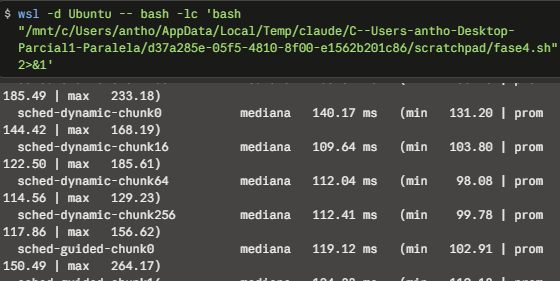
\includegraphics[width=0.95\textwidth]{i7.png}
\caption{Arriba: cierre del barrido en la i5-1035G1 (196 filas de mediciones,
28 corridas registradas). Abajo: barrido de políticas de scheduling en la
i7-11370H, donde se observa \texttt{dynamic} con chunk 16 en 109.64~ms, la
configuración ganadora.}
\end{figure}

%=============================================================================
\section{Conclusiones}

\begin{enumerate}
\item Reestructurar la cola FIFO en fronteras por nivel expone el paralelismo
      sin costo: en el recorrido completo la versión por frontera ya es
      1.33$\times$ más rápida que la cola clásica en la i5 y 1.36$\times$ en la
      i7 antes de paralelizar, por mejor localidad de caché.

\item El CAS atómico sobre un arreglo de marcas resuelve la carrera sin ningún
      \texttt{critical}, y los buffers por hilo eliminan la contención al
      construir la frontera. Las invariantes fueron estables en las 52 corridas
      de ambas máquinas.

\item \texttt{dynamic} con chunk 16 es la mejor política, replicado
      independientemente en dos CPUs. La ganancia es de 8--11\%, no espectacular,
      porque con fronteras de más de un millón de nodos la varianza de grados se
      promedia sola.

\item Las dos optimizaciones que más rindieron no vinieron de la teoría sino de
      medir: una sola región paralela en vez de una por nivel, y reducir el
      arreglo de marcas de 8~MB a 2~MB para que quepa en L3. Esta última mejoró
      la baseline secuencial un 21\% --- es decir, nos \emph{quitó} speedup
      aparente, pero es el número honesto.

\item El resultado final es 2.50$\times$ y 3.21$\times$ sobre 4 núcleos físicos
      en un problema limitado por memoria. Para la consulta puntual X $\to$ Y
      la versión paralela no supera al BFS de cola secuencial, y dejamos la
      causa y la solución documentadas.
\end{enumerate}

\end{document}
